%%
%% This is file `rlhf-for-ir.tex',
%% based on the ACM sigconf template.
%%
%% Commands for TeXCount
%TC:macro \cite [option:text,text]
%TC:macro \citep [option:text,text]
%TC:macro \citet [option:text,text]
%TC:envir table 0 1
%TC:envir table* 0 1
%TC:envir tabular [ignore] word
%TC:envir displaymath 0 word
%TC:envir math 0 word
%TC:envir comment 0 0
%%
\documentclass[sigconf]{acmart}

\AtBeginDocument{%
  \providecommand\BibTeX{{%
    Bib\TeX}}}

\setcopyright{acmlicensed}
\copyrightyear{2026}
\acmYear{2026}
\acmDOI{XXXXXXX.XXXXXXX}
\acmConference[CIKM '26]{ACM International Conference on Information and Knowledge Management}{2026}{TBD}
\acmISBN{978-1-4503-XXXX-X/2026/10}

\usepackage{amsmath}
\usepackage{graphicx}

\begin{document}

\title{Real time Query Steering in Dense Retrieval using RL and Sparse Autoencoders (SAEs)}

\author{Anonymous Author(s)}
\affiliation{%
  \institution{Anonymous Institution}
  \country{}}

\renewcommand{\shortauthors}{Anonymous}

\begin{abstract}
Dense retrieval models suffer from semantic drift (retrieving documents based on spurious distributional overlaps rather than contextual relevance), and correcting this traditionally requires expensive offline fine tuning. We propose Sparse Semantic Steering, a framework that corrects dense retrieval at inference time without retraining the base encoder. We project frozen embeddings through a Sparse Autoencoder (SAE) into a disentangled feature dictionary, then train a Proximal Policy Optimization (PPO) agent over a Context Aware State combining the dense query with top sparse features from a Pseudo Relevance Feedback (PRF) neighborhood. The agent learns bidirectional feature modifications (Negative Semantic Masking), projecting corrections back into the dense index. The policy is trained with simulated implicit feedback from relevance judgments but requires no labels at inference time. On five BEIR datasets the method achieves up to +61.7\% rescue rate (NDCG@10) on ArguAna with negligible overhead (+4.30~MB VRAM, 0.002~ms routing).
\end{abstract}

\begin{CCSXML}
<ccs2012>
 <concept>
  <concept_id>10002951.10003317.10003347.10003350</concept_id>
  <concept_desc>Information systems~Retrieval models and ranking</concept_desc>
  <concept_significance>500</concept_significance>
 </concept>
 <concept>
  <concept_id>10010147.10010257.10010293.10010294</concept_id>
  <concept_desc>Computing methodologies~Neural networks</concept_desc>
  <concept_significance>300</concept_significance>
 </concept>
 <concept>
  <concept_id>10010147.10010257.10010258.10010259</concept_id>
  <concept_desc>Computing methodologies~Reinforcement learning</concept_desc>
  <concept_significance>500</concept_significance>
 </concept>
</ccs2012>
\end{CCSXML}

\ccsdesc[500]{Information systems~Retrieval models and ranking}
\ccsdesc[300]{Computing methodologies~Neural networks}
\ccsdesc[500]{Computing methodologies~Reinforcement learning}

\keywords{dense retrieval, reinforcement learning, sparse autoencoders, semantic steering, information retrieval}

\maketitle

\section{Introduction}

Dense retrieval has become a dominant paradigm in modern information retrieval, superseding the reliance on purely lexical matching by utilizing learned vector representations~\cite{karpukhin2020, izacard2022}. However, dense embeddings can struggle to distinguish fine grained semantic differences, making models vulnerable to hard negatives~\cite{zhan2021}: furthermore, they often fail to generalize across diverse domains, experiencing significant performance drops in zero shot settings due to domain shift~\cite{thakur2021}. Correcting this traditionally requires expensive offline fine tuning over hard negative distributions, a reactive paradigm that scales poorly.

We propose leveraging simulated implicit feedback as an online correction mechanism. User interactions such as skipping top ranked results provide natural implicit preference feedback~\cite{joachims2002}, and formulating this feedback as a reinforcement learning (RL) objective~\cite{afsar2022, christiano2017} offers a principled way to steer queries dynamically. In this work we simulate feedback using benchmark relevance annotations (qrels); deployment with real click logs is a natural extension. However, deploying RL directly over entangled dense spaces is intractable: the continuous action space lacks orthogonal basis directions, preventing agent convergence.

We resolve this by imposing a Sparse Autoencoder (SAE) bottleneck~\cite{huben2024, bricken2023} that projects dense embeddings into a disentangled feature dictionary. A lightweight Proximal Policy Optimization (PPO) agent~\cite{schulman2017} then operates on a Context Aware State combining the dense query with sparse Pseudo Relevance Feedback (PRF) features, learning bidirectional steering (Negative Semantic Masking) to suppress spurious features while a Rank Proportional Scaling Factor protects well performing queries.

Our contributions are:
\begin{enumerate}
\item A sparse semantic steering architecture that transforms the intractable continuous dense perturbation problem into a constrained Markov Decision Process (MDP) over disentangled SAE features;
\item A bidirectional action space with rank proportional torque that enables targeted feature suppression while protecting baseline retrieval quality;
\item Empirical validation on five BEIR datasets showing consistent cross domain improvements (up to +61.7\% rescue rate) with negligible overhead (+4.30~MB Video Random Access Memory (VRAM)).
\end{enumerate}

\begin{figure*}[t]
  \centering
  \includegraphics[width=\textwidth]{rlc-arch.png}
  \caption{The Sparse Semantic Steering pipeline. A frozen dense encoder produces $E_q$, which is projected through an SAE bottleneck into sparse facets. The PPO agent receives a context aware state (top-$k$ active facets from PRF), outputs a bidirectional steering action $\Delta M$, and the corrected query is reranked against the corpus index. The reward is computed from rank changes during training only.}
  \label{fig:architecture}
\end{figure*}

\section{Related Work}

\textbf{RL in Information Retrieval:}
RL has been applied to ranking~\cite{hofmann2013}, query reformulation~\cite{nogueira2017, buck2018}, and recommendation~\cite{afsar2022}. RLHF~\cite{christiano2017} has also been used to align language models~\cite{ouyang2022, stiennon2020}. However, existing RL agents in retrieval operate on discrete token spaces or candidate lists; training a continuous action policy directly on an entangled dense space $\mathbb{R}^d$ yields unstable gradients and sample inefficiency. Continuous vector perturbation in entangled spaces lacks an orthogonal basis for isolating semantic features, causing gradient updates along one direction to corrupt unrelated representational properties.

\textbf{Sparse Autoencoders for Disentanglement:}
Dense embeddings suffer from superposition: networks pack more features than dimensions into almost orthogonal directions~\cite{elhage2022}. Early interpretability work analyzed individual neurons and circuits~\cite{olah2020} or probed feed forward layers as key value memories~\cite{geva2021}, but these methods identify features without enabling targeted intervention on the entangled bases. SAEs address this by projecting activations into overcomplete dictionaries of monosemantic features~\cite{huben2024, bricken2023, templeton2024}. We treat the SAE not as an analytical probe but as a structural tool: it transforms the dense embedding into a disentangled, manipulable sparse vector, converting the intractable continuous steering problem into a constrained MDP.

\textbf{Controllable and Sparse Retrieval:}
Dense retrieval~\cite{karpukhin2020, izacard2022} suffers from semantic drift~\cite{zhan2021}, traditionally corrected via expensive hard negative retraining. Correcting the retrieval manifold via Approximate Nearest Neighbor (ANN) hard negative mining~\cite{xiong2021} is reactive: it shifts embeddings offline but provides no mechanism for inference time correction of individual queries. Sparse models like SPLADE~\cite{formal2021splade} operate over the discrete lexical vocabulary~\cite{robertson1994}, while late interaction architectures like ColBERT~\cite{khattab2020} recover exact match signals by preserving token level dense representations. However, neither paradigm allows for continuous amplification or suppression of abstract, multi token semantic concepts. Our framework bridges this gap by coupling an SAE with an RL agent for continuous semantic steerability.

\section{Method}

Standard dense retrieval scores relevance via Maximum Inner Product Search (MIPS), $S(q,d) = E_Q(q) \cdot E_D(d)$~\cite{johnson2019}. However, high dimensional embeddings suffer from anisotropy~\cite{ethayarajh2019}, and entangled dimensions cause semantic drift: irrelevant documents score above relevant ones. Solving for a direct adjustment $\Delta_q \in \mathbb{R}^d$ in the entangled space is ill posed, as arbitrary continuous shifts destroy unrelated semantic features. We bypass this by formulating correction as an episodic MDP~\cite{sutton2018} over a disentangled sparse basis. Figure~\ref{fig:architecture} illustrates the full pipeline.

\subsection{Sparse State Encoder}

We project frozen dense embeddings $E \in \mathbb{R}^d$ into a sparse space $F \in \mathbb{R}^k$ ($k \gg d$) via an $L_1$-penalized SAE: $F = \text{ReLU}(W_{enc}E + b_{enc})$, $\hat{E} = W_{dec}F + b_{dec}$. The composite loss jointly enforces reconstruction fidelity, sparsity, and inner product preservation:

\begin{equation}
L_{SAE} = \|E - \hat{E}\|_2^2 + \lambda_1 \|F\|_1 + \lambda_2 \sum_{i,j \in \mathcal{B}} (E_i \cdot E_j - \hat{E}_i \cdot \hat{E}_j)^2
\end{equation}

where $\lambda_1 = 1\text{e-}4$ controls sparsity and $\lambda_2 = 1\text{e-}3$ preserves the MIPS ranking topology.

\begin{table*}[t]
  \caption{Cross Domain Retrieval Performance (NDCG@10, inference time state). Bold = best per row.}
  \label{tab:results}
  \begin{tabular}{llccccc}
    \toprule
    Dataset & Domain & SPLADE & ColBERT & Dense Base & RL steered (Ours) & Rescue\\
    \midrule
    SciDocs & Scientific & 0.1395 & 0.1297 & 0.1143 & \textbf{0.1506} & +36.7\%\\
    ArguAna & Argumentative & 0.3588 & 0.3382 & 0.3371 & \textbf{0.4518} & +61.7\%\\
    NFCorpus & Medical & 0.3424 & 0.2923 & 0.2662 & \textbf{0.3595} & +59.6\%\\
    FiQA & Financial & \textbf{0.4655} & 0.4014 & 0.1931 & 0.2755 & +29.1\%\\
    TREC COVID & Bio Medical & \textbf{0.9552} & 0.9244 & 0.3611 & 0.4110 & +87.5\%\\
    \bottomrule
  \end{tabular}
\end{table*}

\subsection{MDP Formulation}

Operating RL on the full 4096-D SAE output would reintroduce dimensionality issues~\cite{lillicrap2016}. We instead extract a compressed, dynamic action space. The top $k{=}10$ retrieved documents are projected through the SAE, and a localized expansion vector is constructed:

\begin{equation}
F_{exp} = F_q + \sum_{i=1}^{k} w_i F_{d_i}
\end{equation}

where weights $w_i$ decay linearly from $1.0$ to $0.1$ by rank, normalized to $\sum w_i = 1$. The top 128 dimensions of $F_{exp}$ define the active semantic facets for the agent.

\textbf{State Space ($\mathcal{S}$):} We define two configurations to separate training supervision from inference:
\textbf{Training state} $s_t^{\text{train}} \in \mathbb{R}^{898}$: the 768-D dense query, a 128-D PRF sparse magnitude vector, a $\log_2$-normalized target rank scalar, and a $\log_2$ rank delta scalar.
\textbf{Inference state} $s_t^{\text{infer}} \in \mathbb{R}^{896}$: only the dense query and PRF magnitudes, with no access to relevance labels or target document identity. All results in this paper use the inference time state exclusively.

\textbf{Action Space ($\mathcal{A}$):} The agent outputs $\Delta M \in [-2.0, 2.0]^{128}$, enabling bidirectional Negative Semantic Masking. The sparse action is projected back via SAE decoder weights, scaled by a Rank Proportional torque:

\begin{equation}
\tau = \max\!\left(0.1, \min\!\left(1.0, \frac{\log_2(\rho_{init})}{\log_2(|\mathcal{C}|)}\right)\right)
\end{equation}

yielding the corrected query: $E_q^{\prime} = E_q + \tau (\Delta M \, W_{dec}^T)$. Well ranked queries ($\rho_{init} \approx 1$) receive near zero correction; poorly ranked queries receive maximal adjustment.

\textbf{Reward Function ($\mathcal{R}$):} Following reward shaping principles~\cite{ng1999}, we construct a Logarithmic Rank Delta Reward from relevance judgments (qrels), simulating implicit feedback~\cite{joachims2002}:

\begin{equation}
R = 10.0 \times (\log_2(\text{Rank}_{old} + 1) - \log_2(\text{Rank}_{new} + 1))
\end{equation}

augmented with discrete bonuses ($+20.0$ for Top~10, $+10.0$ for Top~3). This requires a known relevant document during training only.

\subsection{PPO Optimization}

We optimize the steering policy using PPO~\cite{schulman2017}, an actor critic algorithm~\cite{konda1999} chosen for gradient stability. The Actor $\pi_\theta(a_t|s_t)$ proposes $\Delta M$ and the Critic $V_\phi(s_t)$ reduces variance via Generalized Advantage Estimation (GAE)~\cite{schulman2016}. While PPO's clipped surrogate objective ($\epsilon = 0.2$) is designed to bound policy steps, we rely on its specific code level optimizations to truly prevent destructive updates to the query geometry~\cite{engstrom2020}. Full formulation details are in supplementary materials.

\begin{table}[t]
  \caption{Compute \& VRAM Efficiency.}
  \label{tab:compute}
  \begin{tabular}{lccc}
    \toprule
    Architecture & Params & VRAM & Latency\\
    \midrule
    ColBERT & $\sim$110\,M & High & 15--45\,ms\\
    Dense Base & $\sim$110\,M & Base & 0.001\,ms\\
    RL steered (Ours) & +\,6.56\,M & +\,4.30\,MB & 0.002\,ms\\
    \bottomrule
  \end{tabular}
\end{table}

\section{Experiments}

To evaluate the empirical performance of Sparse Semantic Steering, we conduct a series of retrieval experiments across diverse domains. To support reproducibility, all code, data splits, and pretrained Sparse Autoencoder (SAE) weights are publicly available in our anonymized repository: \url{https://anonymous.4open.science/r/IR-interpretability-RL-ABF2/}.

\subsection{Setup}

We evaluate on five BEIR~\cite{thakur2021} subsets spanning scientific (SciDocs), argumentative (ArguAna), medical (NFCorpus), financial (FiQA), and biomedical (TREC COVID~\cite{voorhees2021}) domains. The base dense encoder (Contriever) is frozen; the steering policy is trained per domain using target dataset relevance labels. We report NDCG@10~\cite{jarvelin2002}. Statistical significance is determined via paired randomized permutation tests ($p < 0.05$)~\cite{smucker2007}. We define \textit{rescue rate} as $(\text{NDCG}_{RL} - \text{NDCG}_{Dense}) / (\text{NDCG}_{SPLADE} - \text{NDCG}_{Dense}) \times 100\%$.

Baselines span three retrieval paradigms: \textbf{Contriever}~\cite{izacard2022} (frozen dense), \textbf{SPLADE v2}~\cite{formal2021spladev2} (learned sparse), and \textbf{ColBERTv2}~\cite{santhanam2022} (late interaction). The SAE is pretrained for 100 epochs using the composite loss (Eq.~1); the PPO agent trains for 300 episodes. Architecture and hyperparameter details are in supplementary materials.

\subsection{Results}

Table~\ref{tab:results} shows results across all five datasets. On abstract reasoning domains (SciDocs, ArguAna, NFCorpus), the steered agent achieves up to +61.7\% rescue rate on ArguAna (0.4518 NDCG@10), outperforming both SPLADE and ColBERT. On jargon-heavy tasks (FiQA, TREC COVID), the method improves over the dense baseline (+87.5\% rescue on TREC COVID) but SPLADE retains the absolute lead. The gap stems from vocabulary coverage: SPLADE's masked-language-model pre-training injects domain-specific lexical tokens (e.g., financial tickers, biomedical MeSH terms) that the frozen Contriever encoder never represented. Sparse steering cannot recover tokens absent from the base encoder's embedding space; it corrects semantic drift within the encoder's representational capacity but cannot synthesize missing vocabulary. Training dynamics (Figure~\ref{fig:dynamics}) confirm the agent converges to a generalized correction strategy rather than memorizing individual queries. As shown in Table~\ref{tab:compute}, the entire pipeline adds only +4.30~MB VRAM and 0.002~ms routing latency (PPO forward pass) over the frozen dense baseline, keeping the same index format and per-document footprint as standard single-vector retrieval.

\textbf{Illustrative Example:} On ArguAna, the query ``Should performance enhancing drugs be accepted in sports?'' ranked the target counter argument at position 112 under the dense baseline, which surfaced documents about general drug criminalization rather than athletic regulation. The steering agent amplified sparse dimensions that, upon post hoc inspection, correspond to competitive fairness (+1.82) and athletic physiology (+1.45), while suppressing dimensions related to narcotics trafficking ($-$1.90) and criminal sentencing ($-$1.55), pushing the target from Rank~112 to Rank~2. These facet labels are assigned post hoc for illustration; systematic interpretability validation is deferred to future work.

\begin{figure}[t]
  \centering
  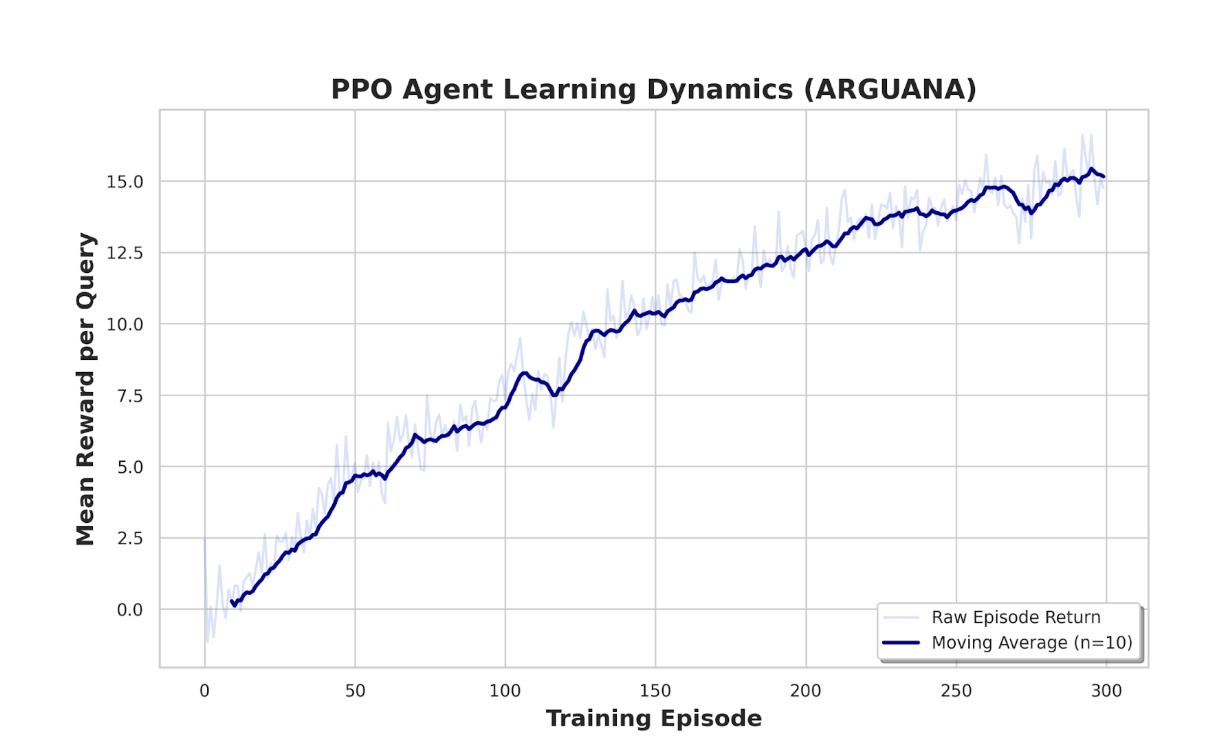
\includegraphics[width=\columnwidth]{fig4.png}
  \caption{PPO agent reward (ArguAna, 300 episodes). The 10-episode moving average increases monotonically, confirming convergence to a generalized correction strategy rather than query memorization.}
  \label{fig:dynamics}
\end{figure}

\subsection{Ablation}

\begin{table}[t]
  \caption{Ablation Studies (ArguAna test split, inference time state).}
  \label{tab:ablation}
  \begin{tabular}{lccc}
    \toprule
    Configuration & NDCG@10 & $\Delta$ & Degrad.\\
    \midrule
    Full Architecture (Ours) & 0.4518 & -- & --\\
    w/o Context Aware State & 0.3522 & -0.0996 & -22.05\%\\
    w/o Negative Masking & 0.4192 & -0.0326 & -7.22\%\\
    w/o Dynamic Torque & 0.4248 & -0.0270 & -5.98\%\\
    Vanilla RL (no SAE) & 0.3277 & -0.1241 & -27.47\%\\
    \bottomrule
  \end{tabular}
\end{table}

Table~\ref{tab:ablation} isolates component contributions. Removing the Context Aware State causes the largest drop ($-22.05\%$): without original query context, the agent applies generic corrections. Operating directly on the dense space without SAE projection (Vanilla RL) yields 0.3277, \textit{below} the frozen Contriever baseline (0.3371), confirming that the disentangled sparse projection is necessary for effective RL-based steering. Negative Masking and Dynamic Torque each contribute meaningfully ($-7.22\%$ and $-5.98\%$). The Vanilla RL result is particularly instructive: without the SAE bottleneck, the agent degrades retrieval below the unmodified baseline, indicating that continuous action RL in entangled dense spaces fails to converge to a useful policy.

\section{Conclusion}

We introduced Sparse Semantic Steering, a framework that corrects semantic drift in dense retrieval at inference time by projecting embeddings through an SAE bottleneck into a disentangled feature space and training a PPO agent to steer queries via bidirectional feature modifications. On five BEIR datasets, the method achieves up to +61.7\% rescue rate on ArguAna, outperforming SPLADE and ColBERT at single-vector speed, with +4.30~MB VRAM and 0.002~ms routing overhead.

\textbf{Deployment Considerations:} Because the dense corpus index is never modified by policy updates, the 6.56M-parameter PPO agent can be retrained on fresh click telemetry and hot swapped at the query router without reindexing. In Retrieval Augmented Generation (RAG) pipelines, the steered retriever functions as a pre generation semantic filter: by suppressing drifted documents before they enter the language model's context window, it reduces downstream hallucination risk without additional inference cost.

\textbf{Limitations:} The reward signal uses benchmark relevance judgments rather than real user interactions; transfer to live click based feedback is untested. The baseline comparison does not include supervised or contextual bandit alternatives. Systematic interpretability evaluation of the sparse features is deferred to future work. The policy is trained per domain; cross domain generalization of a single policy has not been evaluated. Extended formulations, dataset statistics, hyperparameters, and additional analyses are available in the supplementary materials.

\section*{Statement of AI Use}
The authors acknowledge the use of Gemini AI to refine the text, code, and generate the images included in this paper.

\bibliographystyle{ACM-Reference-Format}

\begin{thebibliography}{36}

\bibitem{karpukhin2020}
Vladimir Karpukhin, Barlas O\u{g}uz, Sewon Min, Patrick Lewis, Ledell Wu, Sergey Edunov, Danqi Chen, and Wen-tau Yih. 2020. Dense Passage Retrieval for Open-Domain Question Answering. In \textit{Proceedings of the 2020 Conference on Empirical Methods in Natural Language Processing (EMNLP)}. Association for Computational Linguistics, 6769--6781. \url{https://doi.org/10.18653/v1/2020.emnlp-main.550}

\bibitem{izacard2022}
Gautier Izacard, Mathilde Caron, Lucas Hosseini, Sebastian Riedel, Piotr Bojanowski, Armand Joulin, and Edouard Grave. 2022. Unsupervised Dense Information Retrieval with Contrastive Learning. \textit{Transactions on Machine Learning Research}. \url{https://openreview.net/forum?id=jKN1pXi7b0}

\bibitem{zhan2021}
Jingtao Zhan, Jiaxin Mao, Yiqun Liu, Jiafeng Guo, Min Zhang, and Shaoping Ma. 2021. Optimizing Dense Retrieval Model Training with Hard Negatives. In \textit{Proceedings of the 44th International ACM SIGIR Conference on Research and Development in Information Retrieval}. Association for Computing Machinery, New York, NY, USA, 1503–1512. \url{https://doi.org/10.1145/3404835.3462880}

\bibitem{thakur2021}
Nandan Thakur, Nils Reimers, Andreas R\"uckl\'e, Abhishek Srivastava, and Iryna Gurevych. 2021. BEIR: A Heterogeneous Benchmark for Zero-shot Evaluation of Information Retrieval Models. In \textit{Thirty-fifth Conference on Neural Information Processing Systems Datasets and Benchmarks Track}. \url{https://openreview.net/forum?id=wCu6T5xFjeJ}

\bibitem{joachims2002}
Thorsten Joachims. 2002. Optimizing Search Engines Using Clickthrough Data. In \textit{Proceedings of the Eighth ACM SIGKDD International Conference on Knowledge Discovery and Data Mining} (KDD '02). Association for Computing Machinery, New York, NY, USA, 133–142. \url{https://doi.org/10.1145/775047.775067}

\bibitem{afsar2022}
M. Mehdi Afsar, Trafford Crump, and Behrouz Far. 2022. Reinforcement Learning based Recommender Systems: A Survey. \textit{ACM Computing Surveys} 55, 7, Article 148 (2022), 38 pages. \url{https://doi.org/10.1145/3543846}

\bibitem{christiano2017}
Paul F. Christiano, Jan Leike, Tom Brown, Miljan Martic, Shane Legg, and Dario Amodei. 2017. Deep Reinforcement Learning from Human Preferences. In \textit{Advances in Neural Information Processing Systems}, Vol. 30. Curran Associates, Inc., 4299–4307. \url{https://proceedings.neurips.cc/paper_files/paper/2017/hash/d5e2c0adad503c91f91df240d0cd4e49-Abstract.html}

\bibitem{huben2024}
Robert Huben, Hoagy Cunningham, Logan Riggs Smith, Aidan Ewart, and Lee Sharkey. 2024. Sparse Autoencoders Find Highly Interpretable Features in Language Models. In \textit{The Twelfth International Conference on Learning Representations}. \url{https://openreview.net/forum?id=F76bwRSLeK}

\bibitem{elhage2022}
Nelson Elhage, Tristan Hume, Catherine Olsson, Nicholas Schiefer, Tom Henighan, Shauna Kravec, Zac Hatfield-Dodds, Robert Lasenby, Dawn Drain, Carol Chen, Roger Grosse, Sam McCandlish, Jared Kaplan, Dario Amodei, Martin Wattenberg, and Christopher Olah. 2022. Toy Models of Superposition. \textit{Transformer Circuits Thread}. Retrieved June 6, 2026 from \url{https://transformer-circuits.pub/2022/toy_model/index.html}

\bibitem{bricken2023}
Trenton Bricken, Adly Templeton, Joshua Batson, Brian Chen, Adam Jermyn, Tom Conerly, Nick Turner, Cem Anil, Carson Denison, Amanda Askell, Robert Lasenby, Yifan Wu, Shauna Kravec, Nicholas Schiefer, Tim Maxwell, Nicholas Joseph, Zac Hatfield-Dodds, Alex Tamkin, Karina Nguyen, Brayden McLean, Josiah E Burke, Tristan Hume, Shan Carter, Tom Henighan, and Christopher Olah. 2023. Towards Monosemanticity: Decomposing Language Models With Dictionary Learning. \textit{Transformer Circuits Thread}. Retrieved June 6, 2026 from \url{https://transformer-circuits.pub/2023/monosemantic-features/index.html}

\bibitem{schulman2017}
John Schulman, Filip Wolski, Prafulla Dhariwal, Alec Radford, and Oleg Klimov. 2017. Proximal Policy Optimization Algorithms. \textit{arXiv preprint arXiv:1707.06347}. \url{https://arxiv.org/abs/1707.06347}

\bibitem{hofmann2013}
Katja Hofmann, Shimon Whiteson, and Maarten de Rijke. 2013. Balancing Exploration and Exploitation in Listwise and Pairwise Online Learning to Rank for Information Retrieval. \textit{Information Retrieval}, 16(1), 63--90. \url{https://doi.org/10.1007/s10791-012-9197-9}

\bibitem{nogueira2017}
Rodrigo Nogueira and Kyunghyun Cho. 2017. Task-Oriented Query Reformulation with Reinforcement Learning. In \textit{Proceedings of the 2017 Conference on Empirical Methods in Natural Language Processing}. Association for Computational Linguistics, 574–583. \url{https://aclanthology.org/D17-1061/}

\bibitem{buck2018}
Christian Buck, Jannis Bulian, Massimiliano Ciaramita, Wojciech Gajewski, Andrea Gesmundo, Neil Houlsby, and Wei Wang. 2018. Ask the Right Questions: Active Question Reformulation with Reinforcement Learning. In \textit{The Sixth International Conference on Learning Representations}. \url{https://openreview.net/forum?id=S1CChZ-CZ}

\bibitem{ouyang2022}
Long Ouyang, Jeffrey Wu, Xu Jiang, Diogo Almeida, Carroll L. Wainwright, Pamela Mishkin, Chong Zhang, Sandhini Agarwal, Katarina Slama, Alex Ray, John Schulman, Jacob Hilton, Fraser Kelton, Luke Miller, Maddie Simens, Amanda Askell, Peter Welinder, Paul Christiano, Jan Leike, and Ryan Lowe. 2022. Training Language Models to Follow Instructions with Human Feedback. In \textit{Advances in Neural Information Processing Systems}, Vol. 35. Curran Associates, Inc., 27730–27744. \url{https://proceedings.neurips.cc/paper_files/paper/2022/hash/b1efde53be364a73914f58805a001731-Abstract-Conference.html}

\bibitem{stiennon2020}
Nisan Stiennon, Long Ouyang, Jeffrey Wu, Daniel Ziegler, Ryan Lowe, Chelsea Voss, Alec Radford, Dario Amodei, and Paul F. Christiano. 2020. Learning to Summarize with Human Feedback. In \textit{Advances in Neural Information Processing Systems}, Vol. 33. Curran Associates, Inc., 3008–3021. \url{https://proceedings.neurips.cc/paper/2020/hash/1f89885d556929e98d3ef9b86448f951-Abstract.html}

\bibitem{olah2020}
Chris Olah, Nick Cammarata, Ludwig Schubert, Gabriel Goh, Michael Petrov, and Shan Carter. 2020. Zoom In: An Introduction to Circuits. \textit{Distill}. \url{https://doi.org/10.23915/distill.00024.001}

\bibitem{geva2021}
Mor Geva, Roei Schuster, Jonathan Berant, and Omer Levy. 2021. Transformer Feed-Forward Layers Are Key-Value Memories. In \textit{Proceedings of the 2021 Conference on Empirical Methods in Natural Language Processing}. Association for Computational Linguistics, 5484–5495. \url{https://aclanthology.org/2021.emnlp-main.446/}

\bibitem{templeton2024}
Adly Templeton, Tom Conerly, Jonathan Marcus, Jack Clark, Saurav Kadavath, Sam McCandlish, Tom Henighan, Tristan Hume, Zac Hatfield-Dodds, Robert Lasenby, Jared Kaplan, and Chris Olah. 2024. Scaling Monosemanticity: Extracting Interpretable Features from Claude 3 Sonnet. \textit{Transformer Circuits Thread}. Retrieved June 6, 2026 from \url{https://transformer-circuits.pub/2024/scaling-monosemanticity/index.html}

\bibitem{xiong2021}
Lee Xiong, Chenyan Xiong, Ye Li, Kwok-Fung Tang, Jialin Liu, Paul N. Bennett, Junaid Ahmed, and Arnold Overwijk. 2021. Approximate Nearest Neighbor Negative Contrastive Learning for Dense Text Retrieval. In \textit{The Ninth International Conference on Learning Representations}. \url{https://openreview.net/forum?id=zeFrfgyZln}

\bibitem{formal2021splade}
Thibault Formal, Benjamin Piwowarski, and St\'ephane Clinchant. 2021. SPLADE: Sparse Lexical and Expansion Model for First Stage Ranking. In \textit{Proceedings of the 44th International ACM SIGIR Conference on Research and Development in Information Retrieval}. Association for Computing Machinery, 2288–2292. \url{https://doi.org/10.1145/3404835.3463098}

\bibitem{khattab2020}
Omar Khattab and Matei Zaharia. 2020. ColBERT: Efficient and Effective Passage Search via Contextualized Late Interaction over BERT. In \textit{Proceedings of the 43rd International ACM SIGIR Conference on Research and Development in Information Retrieval}. Association for Computing Machinery, 39–48. \url{https://doi.org/10.1145/3397271.3401075}

\bibitem{robertson1994}
Stephen E. Robertson and Steve Walker. 1994. Some Simple Effective Approximations to the 2-Poisson Model for Probabilistic Weighted Retrieval. In \textit{Proceedings of the 17th Annual International ACM SIGIR Conference on Research and Development in Information Retrieval}. Springer, 232–241. \url{https://doi.org/10.1007/978-1-4471-2099-5_24}

\bibitem{johnson2019}
Jeff Johnson, Matthijs Douze, and Herv\'{e} J\'{e}gou. 2019. Billion-Scale Similarity Search with GPUs. \textit{IEEE Transactions on Big Data}, 7(3), 535--547. \url{https://doi.org/10.1109/TBDATA.2019.2921572}

\bibitem{ethayarajh2019}
Kawin Ethayarajh. 2019. How Contextual are Contextualized Word Representations? Comparing the Geometry of BERT, ELMo, and GPT-2 Embeddings. In \textit{Proceedings of the 2019 Conference on Empirical Methods in Natural Language Processing and the 9th International Joint Conference on Natural Language Processing (EMNLP-IJCNLP)}. Association for Computational Linguistics, 55–65. \url{https://aclanthology.org/D19-1006/}

\bibitem{sutton2018}
Richard S. Sutton and Andrew G. Barto. 2018. \textit{Reinforcement Learning: An Introduction} (2nd ed.). MIT Press, Cambridge, MA.

\bibitem{lillicrap2016}
Timothy P. Lillicrap, Jonathan J. Hunt, Alexander Pritzel, Nicolas Heess, Tom Erez, Yuval Tassa, David Silver, and Daan Wierstra. 2016. Continuous Control with Deep Reinforcement Learning. In \textit{The 4th International Conference on Learning Representations}. \url{https://arxiv.org/abs/1509.02971}

\bibitem{ng1999}
Andrew Y. Ng, Daishi Harada, and Stuart Russell. 1999. Policy Invariance Under Reward Transformations: Theory and Application to Reward Shaping. In \textit{Proceedings of the 16th International Conference on Machine Learning}. Morgan Kaufmann Publishers Inc., 278–287. \url{https://dl.acm.org/doi/10.5555/645528.657613}

\bibitem{konda1999}
Vijay R. Konda and John N. Tsitsiklis. 1999. Actor-Critic Algorithms. In \textit{Advances in Neural Information Processing Systems}, Vol. 12. MIT Press, 1008–1014. \url{https://proceedings.neurips.cc/paper/1999/hash/6449f44a102fde848669bdd9eb6b76fa-Abstract.html}

\bibitem{schulman2016}
John Schulman, Philipp Moritz, Sergey Levine, Michael I. Jordan, and Pieter Abbeel. 2016. High-Dimensional Continuous Control Using Generalized Advantage Estimation. In \textit{The 4th International Conference on Learning Representations}. \url{https://arxiv.org/abs/1506.02438}

\bibitem{engstrom2020}
Logan Engstrom, Andrew Ilyas, Shibani Santurkar, Dimitris Tsipras, Firdaus Janoos, Larry Rudolph, and Aleksander M\k{a}dry. 2020. Implementation Matters in Deep Policy Gradients: A Case Study on PPO and TRPO. In \textit{The Eighth International Conference on Learning Representations}. \url{https://openreview.net/forum?id=r1etN1rtPB}

\bibitem{voorhees2021}
Ellen Voorhees, Tasmeer Alam, Steven Bedrick, Dina Demner-Fushman, William R. Hersh, Kyle Lo, Kirk Roberts, Ian Soboroff, and Lucy Lu Wang. 2021. TREC-COVID: Constructing a Pandemic Information Retrieval Test Collection. \textit{SIGIR Forum}, 54(1), 1–12. \url{https://doi.org/10.1145/3451964.3451965}

\bibitem{jarvelin2002}
Kalervo J\"arvelin and Jaana Kek\"al\"ainen. 2002. Cumulated Gain-Based Evaluation of IR Techniques. \textit{ACM Transactions on Information Systems}, 20(4), 422–446. \url{https://doi.org/10.1145/582415.582418}

\bibitem{smucker2007}
Mark D. Smucker, James Allan, and Ben Carterette. 2007. A Comparison of Statistical Significance Tests for Information Retrieval Evaluation. In \textit{Proceedings of the 16th ACM International Conference on Information and Knowledge Management}. Association for Computing Machinery, 623–632. \url{https://doi.org/10.1145/1321440.1321528}

\bibitem{formal2021spladev2}
Thibault Formal, Carlos Lassance, Benjamin Piwowarski, and St\'ephane Clinchant. 2021. SPLADE v2: Sparse Lexical and Expansion Model for Information Retrieval. \textit{arXiv preprint arXiv:2109.10086}. \url{https://arxiv.org/abs/2109.10086}

\bibitem{santhanam2022}
Keshav Santhanam, Omar Khattab, Jon Saad-Falcon, Christopher Potts, and Matei Zaharia. 2022. ColBERTv2: Effective and Efficient Retrieval via Lightweight Late Interaction. In \textit{Proceedings of the 2022 Conference of the North American Chapter of the Association for Computational Linguistics: Human Language Technologies}. Association for Computational Linguistics, 3715–3734. \url{https://aclanthology.org/2022.naacl-main.272}

\end{thebibliography}

\end{document}
